\documentclass[12pt]{article}\usepackage[]{graphicx}\usepackage[]{color}
% maxwidth is the original width if it is less than linewidth
% otherwise use linewidth (to make sure the graphics do not exceed the margin)
\makeatletter
\def\maxwidth{ %
  \ifdim\Gin@nat@width>\linewidth
    \linewidth
  \else
    \Gin@nat@width
  \fi
}
\makeatother

\definecolor{fgcolor}{rgb}{0.345, 0.345, 0.345}
\newcommand{\hlnum}[1]{\textcolor[rgb]{0.686,0.059,0.569}{#1}}%
\newcommand{\hlstr}[1]{\textcolor[rgb]{0.192,0.494,0.8}{#1}}%
\newcommand{\hlcom}[1]{\textcolor[rgb]{0.678,0.584,0.686}{\textit{#1}}}%
\newcommand{\hlopt}[1]{\textcolor[rgb]{0,0,0}{#1}}%
\newcommand{\hlstd}[1]{\textcolor[rgb]{0.345,0.345,0.345}{#1}}%
\newcommand{\hlkwa}[1]{\textcolor[rgb]{0.161,0.373,0.58}{\textbf{#1}}}%
\newcommand{\hlkwb}[1]{\textcolor[rgb]{0.69,0.353,0.396}{#1}}%
\newcommand{\hlkwc}[1]{\textcolor[rgb]{0.333,0.667,0.333}{#1}}%
\newcommand{\hlkwd}[1]{\textcolor[rgb]{0.737,0.353,0.396}{\textbf{#1}}}%
\let\hlipl\hlkwb

\usepackage{framed}
\makeatletter
\newenvironment{kframe}{%
 \def\at@end@of@kframe{}%
 \ifinner\ifhmode%
  \def\at@end@of@kframe{\end{minipage}}%
  \begin{minipage}{\columnwidth}%
 \fi\fi%
 \def\FrameCommand##1{\hskip\@totalleftmargin \hskip-\fboxsep
 \colorbox{shadecolor}{##1}\hskip-\fboxsep
     % There is no \\@totalrightmargin, so:
     \hskip-\linewidth \hskip-\@totalleftmargin \hskip\columnwidth}%
 \MakeFramed {\advance\hsize-\width
   \@totalleftmargin\z@ \linewidth\hsize
   \@setminipage}}%
 {\par\unskip\endMakeFramed%
 \at@end@of@kframe}
\makeatother

\definecolor{shadecolor}{rgb}{.97, .97, .97}
\definecolor{messagecolor}{rgb}{0, 0, 0}
\definecolor{warningcolor}{rgb}{1, 0, 1}
\definecolor{errorcolor}{rgb}{1, 0, 0}
\newenvironment{knitrout}{}{} % an empty environment to be redefined in TeX

\usepackage{alltt}


\usepackage[hmargin=1in,vmargin=1in]{geometry}
\usepackage{parskip}
\usepackage{hyperref}
\usepackage{graphicx}
\hypersetup{pdfstartview=FitV,hidelinks}




\IfFileExists{upquote.sty}{\usepackage{upquote}}{}
\begin{document}

{
  \Large
  \centering
  Lab 3 Assignment --- Stochasticity and Extinction \\
  Due before Monday \par
}

{\bf Random Numbers in Excel \\}


\begin{figure}[h]
  \centering
  \fbox{
    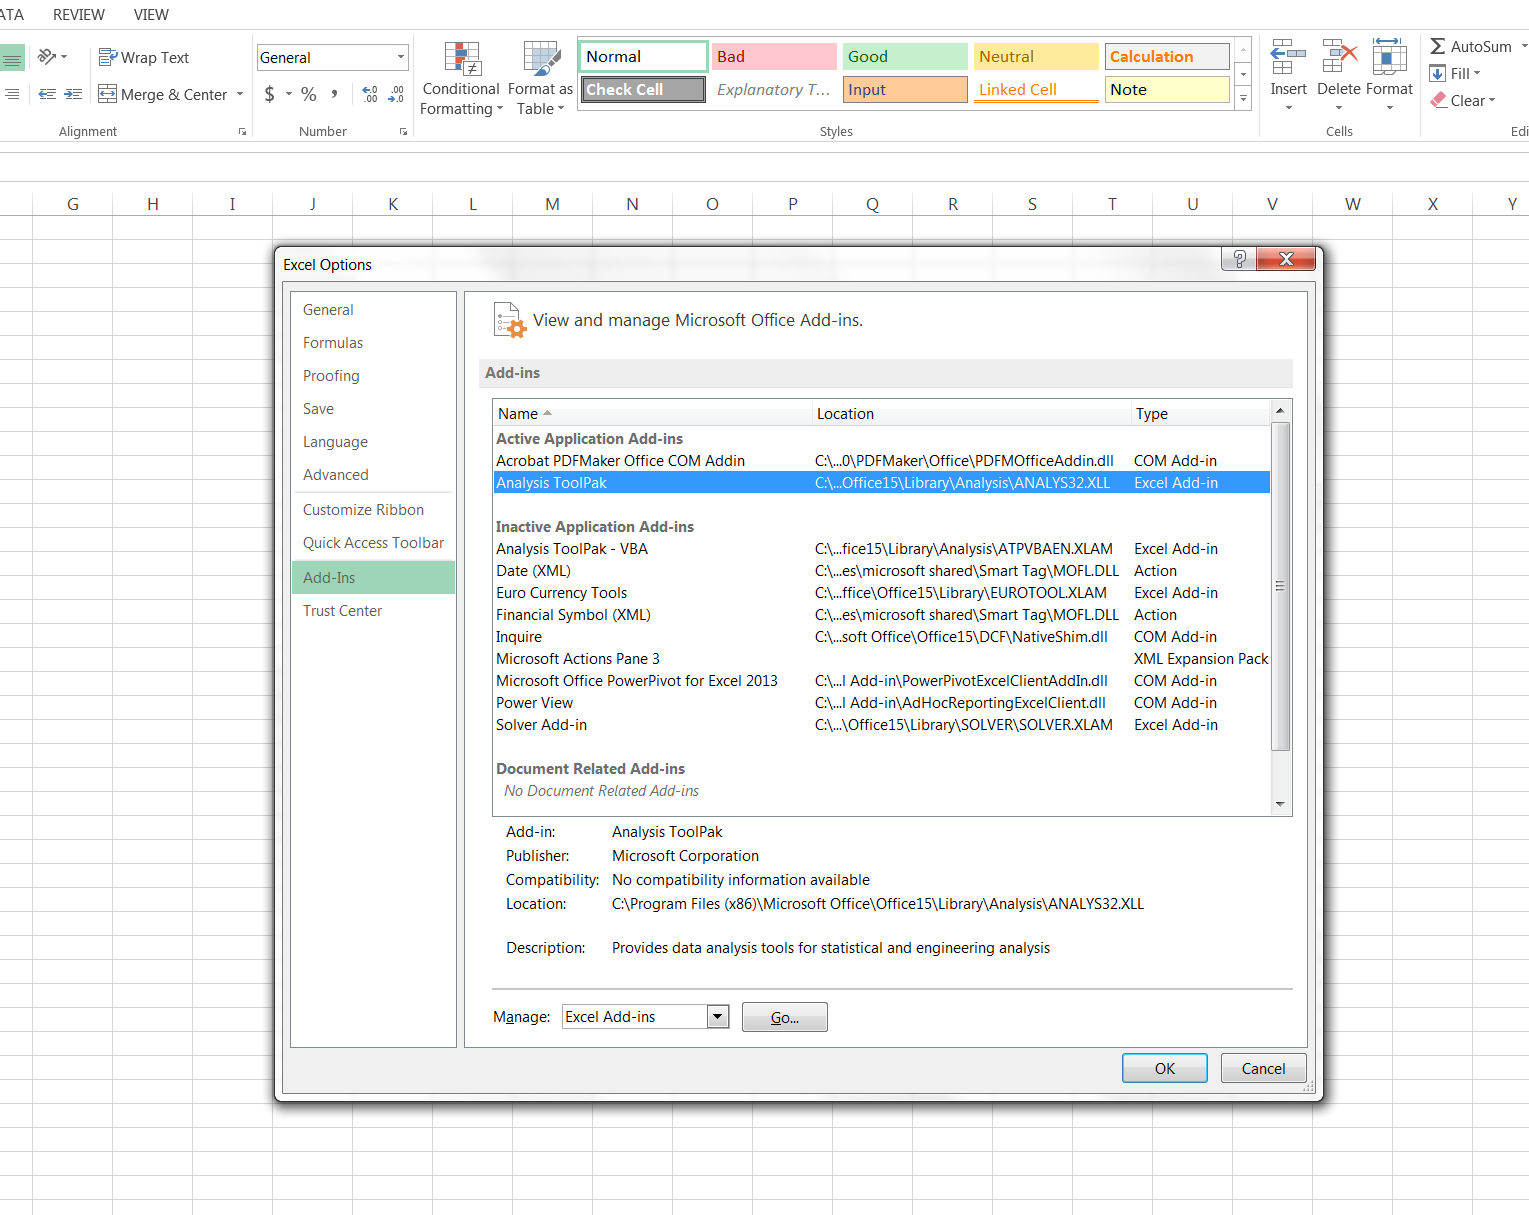
\includegraphics[width=\textwidth]{figs/Excel-RNG}
  }
  \caption{To generate random numbers in Excel, you must load the
    ``Analysis Toolpak'' add-in by clicking
    {\tt File $>$ Options $>$ Add-Ins $>$ Analysis Toolpak}. Then hit
    ``Go'' (not ``OK'') and select ``Analysis Tookpak'' again.}
  \label{fig:rng}
\end{figure}

\clearpage

\begin{figure}[h]
  \centering
  \fbox{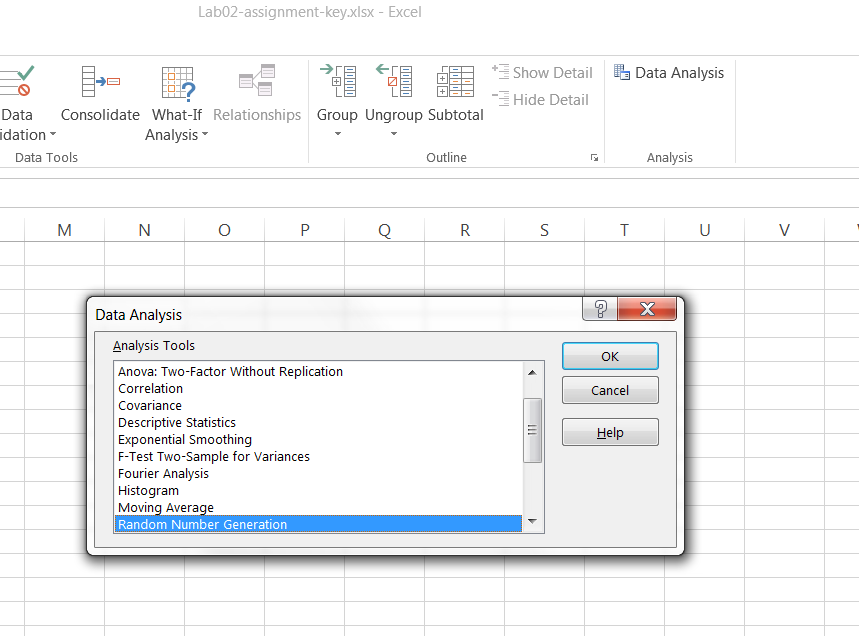
\includegraphics[width=0.6\textwidth]{figs/Excel-RNG-2}}
  \caption{\footnotesize Once the Analysis ToolPak is installed, you can generate
    random numbers by clicking the ``Data Analysis'' button in the
    ``Data'' tab.
  }
  \label{fig:rng-2}
\end{figure}

\vspace{1cm}

\begin{figure}[h]
  \centering
  \fbox{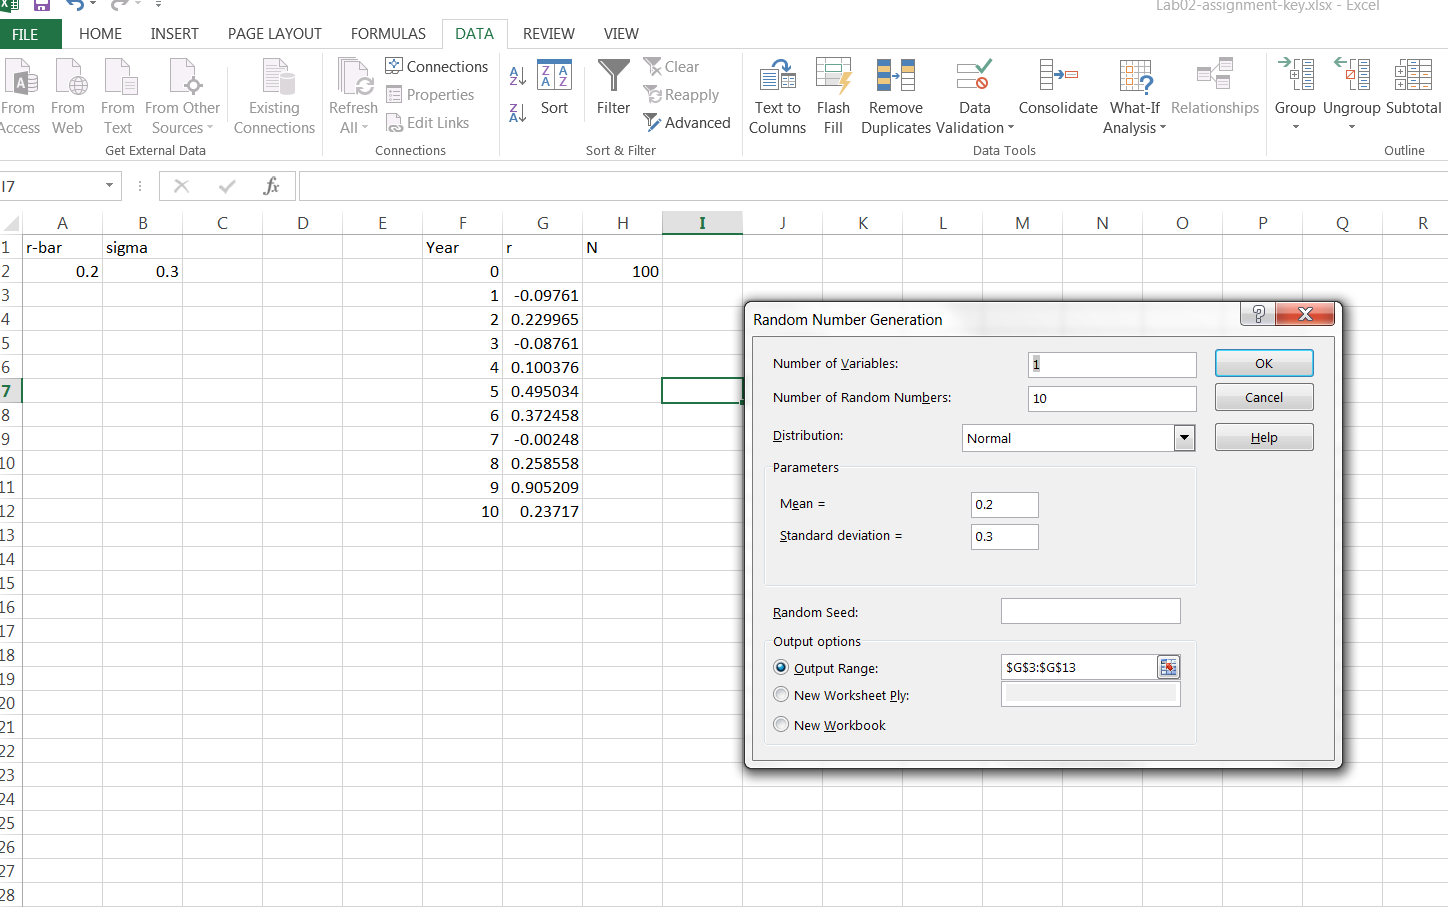
\includegraphics[width=0.6\textwidth]{figs/Excel-RNG-3}}
  \caption{\footnotesize We will use three distributions: Normal,
    Binomial, and Poisson. The latter two are only used in Exercise
    III. Note: You can think of the ``number of variables'' as the
    number of columns of random variables, and the ``number of random
    numbers'' as the number of cells in each column.
  }
  \label{fig:rng-3}
\end{figure}


\clearpage

Answer each of the following questions and upload your completed Excel
file and R script to ELC. Be sure to show your calculations. \\

\vspace{12pt}

{\bf Exercise I \\}
\begin{enumerate}
  \item Suppose a population is growing geometrically with
    $r=-0.2$ and $N_0=500$. There is no random variation, and
    quasi-extinction occurs when $N$ falls below 20 individuals.
    What is the time to quasi-extinction ($T_e$)? In other words, how
    long will it take for the population to fall below 20 individuals?
  \item Now imagine that there is no demographic stochasticity,
    but environmental stochasticity occurs with $X_t \sim
    \mathrm{Normal}(\mu=0, \sigma=10)$, where $\mu$ is the mean
    and $\sigma$ is the standard deviation of the random variable
    $X$. Generate the random values of $X$ that will be
    used in the 10 simulations in the next step.
  \item Conduct 10 simulations over a 30 year time period, and force
    the population size to zero after it falls below the threshold.
    This can be done by multiplying the
    growth equation by a ``test statement'', like this:
    {\tt =(EQUATION)*(CELL>20)}, where {\tt EQUATION} should be
    replaced with the population growth equation and {\tt CELL} should
    be replaced with the cell reference for abundance at the previous
    time step. Plot the projections.
  \item What is the average $T_e$ based on these 10 simulations?
\end{enumerate}

\vspace{12pt}


{\bf Exercise II \\}
\begin{enumerate}
  \item Simulate 10 populations under a logistic growth model with
    $N_0$=20, $K$=40, and a normally-distributed growth rate $r_{\mathrm{max}_t}
    \sim \mathrm{Norm}(\mu=0.1, \sigma=0.2)$. Assume that the
    quasi-extinction threshold is equal to 10, and force the
    population size to zero if it falls below the threshold using a
    test statement as before. Plot the projections.
  \item What are the quasi-extinction risks at years 5, 10, and 15?
\end{enumerate}


\newpage


{\bf Exercise III \\ }
In this exercise, you will be exposed to two new probability
distributions: the Poisson and the binomial. The Poisson distribution
is useful for data that are non-negative integers. It only has
a single parameter (often called ``lambda'' but not to be confused with the
finite rate of increase) that describes the expected value of the
count data. In stochastic population models, the Poisson distribution
can be used to model the number of births ($B_t$) that occur in a time
interval. 

The binomial distribution is also useful for data that are
non-negative integers, but it has an upper bound. In population
models, the upper bound is often population size, and we use the model
to describe how many individuals die during some time period.

Assume that a population is geographically closed such that there is
no immigration or emigration. The number of individuals born is a
Poisson random variable:
\[
  B_t \sim \mathrm{Poisson}(N_t \times b)
\]
and the number that die each year is a binomial random variable:
\[
  D_t \sim \mathrm{Binomial}(N_t, d)
\]
Abundance is just the number that were alive plus the number that were
born, minus the number that died:
\[
  N_{t+1} = N_t + B_t - D_t
\]
\begin{enumerate}
  \item Beginning with $N_0=300$, conduct one simulation over 5
    years, in which $b=0.3$ and $d=0.2$. Plot the simulated values of
    abundance over time. Hint: You have  
    to randomly generate $B_t$ and $D_t$ each year before you can compute
    $N_t$.
  \item Do you think this population will reach a stochastic
    equilibrium? Why or why not? (A stochastic equilibrium occurs when
    a population fluctuates around a long-term average).
  \item Can population size ever be less than zero under this model?
    Why or why not?
  \item Do another simulation, but this time make the mortality rate
    ($d$) density-dependent according to the model $d_t = 0.2 +
    0.001\times N_t$. Will this population reach a stochastic equilibrium? If
    so, at what value of abundance does the equilibrium point occur?
\end{enumerate}


\newpage

{\bf Example {\tt R} code \\}



Geometric growth with environmental stochasticity



\begin{knitrout}
\definecolor{shadecolor}{rgb}{0.969, 0.969, 0.969}\color{fgcolor}\begin{kframe}
\begin{alltt}
\hlstd{r} \hlkwb{<-} \hlnum{0.01}
\hlstd{sigma} \hlkwb{<-} \hlnum{5}
\hlstd{nYears} \hlkwb{<-} \hlnum{50}
\hlstd{N1} \hlkwb{<-} \hlkwd{rep}\hlstd{(}\hlnum{NA}\hlstd{, nYears)}  \hlcom{## Empty vector for population size }
\hlstd{X} \hlkwb{<-} \hlkwd{rep}\hlstd{(}\hlnum{NA}\hlstd{, nYears)}   \hlcom{## Random variable for environmental stochasticity}
\hlstd{N1[}\hlnum{1}\hlstd{]} \hlkwb{<-} \hlnum{100}           \hlcom{## Initial population size}
\hlkwa{for}\hlstd{(t} \hlkwa{in} \hlnum{2}\hlopt{:}\hlstd{nYears) \{}
    \hlstd{X[t]} \hlkwb{<-} \hlkwd{rnorm}\hlstd{(}\hlkwc{n}\hlstd{=}\hlnum{1}\hlstd{,} \hlkwc{mean}\hlstd{=}\hlnum{0}\hlstd{,} \hlkwc{sd}\hlstd{=sigma)}
    \hlstd{N1[t]} \hlkwb{<-} \hlstd{N1[t}\hlopt{-}\hlnum{1}\hlstd{]} \hlopt{+} \hlstd{N1[t}\hlopt{-}\hlnum{1}\hlstd{]}\hlopt{*}\hlstd{r} \hlopt{+} \hlstd{X[t]}
\hlstd{\}}
\hlkwd{plot}\hlstd{(}\hlnum{1}\hlopt{:}\hlstd{nYears, N1,} \hlkwc{xlab}\hlstd{=}\hlstr{"Time"}\hlstd{,} \hlkwc{ylab}\hlstd{=}\hlstr{"Abundance"}\hlstd{,} \hlkwc{type}\hlstd{=}\hlstr{"b"}\hlstd{)}
\end{alltt}
\end{kframe}

{\centering \includegraphics[width=0.9\textwidth]{figure/geom-stoch-1} 

}


\end{knitrout}


\newpage

Poisson-Binomial birth-death model

\begin{knitrout}
\definecolor{shadecolor}{rgb}{0.969, 0.969, 0.969}\color{fgcolor}\begin{kframe}
\begin{alltt}
\hlstd{b} \hlkwb{<-} \hlnum{0.15}  \hlcom{## Birth rate}
\hlstd{d} \hlkwb{<-} \hlnum{0.2}   \hlcom{## Mortality rate}
\hlstd{nYears} \hlkwb{<-} \hlnum{50}
\hlstd{N2} \hlkwb{<-} \hlkwd{rep}\hlstd{(}\hlnum{NA}\hlstd{, nYears)}  \hlcom{## Empty vector for population size }
\hlstd{B} \hlkwb{<-} \hlkwd{rep}\hlstd{(}\hlnum{NA}\hlstd{, nYears)}   \hlcom{## Random variable for nBirths}
\hlstd{D} \hlkwb{<-} \hlkwd{rep}\hlstd{(}\hlnum{NA}\hlstd{, nYears)}   \hlcom{## Random variable for nDeaths}
\hlstd{N2[}\hlnum{1}\hlstd{]} \hlkwb{<-} \hlnum{100}           \hlcom{## Initial population size}
\hlkwa{for}\hlstd{(t} \hlkwa{in} \hlnum{2}\hlopt{:}\hlstd{nYears) \{}
    \hlstd{B[t}\hlopt{-}\hlnum{1}\hlstd{]} \hlkwb{<-} \hlkwd{rpois}\hlstd{(}\hlkwc{n}\hlstd{=}\hlnum{1}\hlstd{,} \hlkwc{lambda}\hlstd{=N2[t}\hlopt{-}\hlnum{1}\hlstd{]}\hlopt{*}\hlstd{b)}
    \hlstd{D[t}\hlopt{-}\hlnum{1}\hlstd{]} \hlkwb{<-} \hlkwd{rbinom}\hlstd{(}\hlkwc{n}\hlstd{=}\hlnum{1}\hlstd{,} \hlkwc{size}\hlstd{=N2[t}\hlopt{-}\hlnum{1}\hlstd{],} \hlkwc{prob}\hlstd{=d)}
    \hlstd{N2[t]} \hlkwb{<-} \hlstd{N2[t}\hlopt{-}\hlnum{1}\hlstd{]} \hlopt{+} \hlstd{B[t}\hlopt{-}\hlnum{1}\hlstd{]} \hlopt{-} \hlstd{D[t}\hlopt{-}\hlnum{1}\hlstd{]}
\hlstd{\}}
\hlkwd{plot}\hlstd{(}\hlnum{1}\hlopt{:}\hlstd{nYears, N2,} \hlkwc{xlab}\hlstd{=}\hlstr{"Time"}\hlstd{,} \hlkwc{ylab}\hlstd{=}\hlstr{"Abundance"}\hlstd{,} \hlkwc{type}\hlstd{=}\hlstr{"b"}\hlstd{)}
\end{alltt}
\end{kframe}

{\centering \includegraphics[width=0.9\textwidth]{figure/pois-bin-1} 

}


\end{knitrout}


\end{document}

